
%\newmdtheoremenv{definition}{Definition}
%\newmdtheoremenv{theorem}{Theorem}
%\newmdtheoremenv{lemma}{Lemma}






\section{Formulating a Mathematical Model}
	\subsection{Network Topology}
	\begin{frame}
		Incidence Matrix $A = (a_{ij}) \in \mathbb{R}^{k \times l}$:
		\begin{displaymath}
			\tilde{a}_{ij} = 
			\begin{cases}
				1 &   \text{edge $j$ starts at node $i$},\\
				-1 &  \text{edge $j$  ends at node $i$},\\
				0 & \text{else}.				
			\end{cases}
		\end{displaymath}
		With $\mathcal{N} = (n_0, n_1, n_2, ..., n_k)$ nodes and $\mathcal{E} = \{e_{j}: j = 1,...,l\}$ edges, where $|\mathcal{N}| = k$ is the number of nodes and $|\mathcal{E}| = l$ \\
		$u = (u_0, u_1, u_2, ...)$ the corresponding electrical potentials to the nodes.\\
		$\to$ reduced incidence matrix
	\end{frame}

	\subsection{Energy Conservation Laws}
	\begin{frame}
		\begin{itemize}
			\item \textbf{Kirchhoff's voltage law (KVL):} \newline
			The sum of voltages along each loop of the network must equal to zero. Using the incidence matrix $A$ this law can be formulated as
			\begin{equation}
				\label{KVL}
				A^\top  u = v.
			\end{equation}
			\item \textbf{Kirchhoff's current law (KCL):} \newline
			For any node, the sum of currents flowing into the node is equal to the sum of currents flowing out of the node. Using the incidence matrix $A$ again, this law can be formulated as
			\begin{equation}
				\label{KCL}
				A  i = 0.
			\end{equation}
		\end{itemize}
	\end{frame}

	\subsection{Electrical Components and their Relations}
		
	\begin{frame}
		\begin{itemize}
			\item \textbf{Resistor} \newline
			\begin{equation}
				\label{eq:resistor law}
				v = R \ i \quad \text{or} \quad i = G \ u.
			\end{equation}
			\begin{figure}[H]
				\label{fig:resistor symbol}
				\centering
				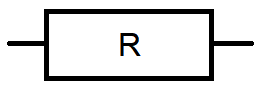
\includegraphics[width=2cm]{../Tex/pictures/resistor.png}
				\caption{resistor symbol}
			\end{figure}
			
			\item \textbf{Capacitor} \newline
			\begin{equation}
				\label{eq:capacitor law}
				Q = C \ v \quad \text{and by derivation in t} \quad I = C \ \frac{d}{dt}v = C \ v'.
			\end{equation}
			\begin{figure}[H]
				\label{fig:capacitor symbol}
				\centering
				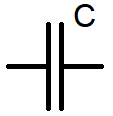
\includegraphics[width=2cm]{../Tex/pictures/capacitor.png}
				\caption{capacitor symbol}
			\end{figure}
		\end{itemize}
	\end{frame}
			
	\begin{frame}	
		\begin{itemize}
			\item \textbf{Inductor (Coil)} \newline
			\begin{equation}
				\label{eq:inductor law}
				\Phi = L \ i \quad \text{and by derivation in t} \quad v = L \ i'.
			\end{equation}
			\begin{figure}[H]
				\label{fig:inductor symbol}
				\centering
				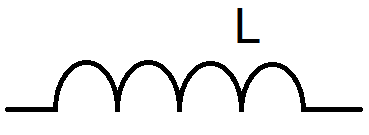
\includegraphics[width=3cm]{../Tex/pictures/inductance.png}
				\caption{inductor symbol}
			\end{figure}
			
			\item \textbf{Voltage Source} \newline
			\begin{equation}
				\label{eq:voltage source law}
				v = v_{src}
			\end{equation}
			\begin{figure}[H]
				\label{fig:voltage source symbol}
				\centering
				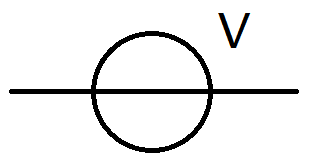
\includegraphics[width=4cm]{../Tex/pictures/voltage_source.png}
				\caption{voltage source symbol}
			\end{figure}
		\end{itemize}
	\end{frame}
			
	\begin{frame}
		\begin{itemize}
			\item \textbf{Current Source} \newline
			\begin{equation}
				\label{eq:current source law}
				i = i_{src}
			\end{equation}
			\begin{figure}[H]
				\label{fig:current source symbol}
				\centering
				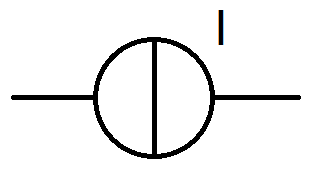
\includegraphics[width=4cm]{../Tex/pictures/current_source.png}
				\caption{current source symbol}
			\end{figure}
		\end{itemize}
	\end{frame}

	\subsection{Modified Nodal Analysis - MNA}
	\begin{frame}
		\begin{equation}
			\label{MNA_Matrixform}
			\begin{pmatrix}
				A_C C A_C^\top & 0 & 0 \\
				0 & L & 0 \\
				0 & 0 & 0
			\end{pmatrix}
			*
			\begin{pmatrix}
				u' \\
				i_L' \\
				i_V'
			\end{pmatrix}
			+
			\begin{pmatrix}
				A_R G A_R^\top & A_L & A_V \\
				-A_L^\top & 0 & 0 \\
				-A_V^\top & 0 & 0 
			\end{pmatrix}
			*
			\begin{pmatrix}
				u \\
				i_L \\
				i_V
			\end{pmatrix}
			=
			\begin{pmatrix}
				-A_I i_{src} \\
				0 \\
				-v_{src}
			\end{pmatrix} , 
		\end{equation}
	\end{frame}

\section{Differential Algebraic Equations}
	\subsection{Types of DAEs}
	\begin{frame}
		In the most general form a DAE can be written as:
		Find $y:\mathbb{R} \to \mathbb{R}^n$ such that
		\begin{equation}
			\label{Abstract_DAE}
			F(t, y(t), y'(t)) = 0, \qquad \forall t \in I
		\end{equation}
		
		with $F:\mathbb{R} \times \mathbb{R}^n \times \mathbb{R}^n \to \mathbb{R}^n$ sufficiently smooth and $I$ the time-interval.
	\end{frame}
	\begin{frame}
		\begin{itemize}
			\item \textbf{Linear systems with constant coeffiecients} \newline
			are systems of the form: find $y$ such that
			\begin{equation}
				\label{DAE-const-coeff}
				A y'(t) + B y(t) = f(t) ,
			\end{equation}
			with $A,B \in \mathbb{R}^{n \times n}$, $A$ singular, $B$ regular and $f:\mathbb{R} \to \mathbb{R}^n$ a function in time.
			
			\item \textbf{Linear time dependent systems}
			are systems of the form: find $y$ such that
			\begin{displaymath}
				A(t) y'(t) + B(t) y(t) = f(t) ,
			\end{displaymath}
			with $A, B:\mathbb{R} \to \mathbb{R}^{n \times n}$, $f:\mathbb{R} \to \mathbb{R}^n$ functions, such that for every $t \in \mathbb{R}$ the matrix $A(t)$ is singular and the matrix $B(t)$ regular.
			
			\item  \textbf{Structured (non-linear) systems} \newline
			are semi-explicit systems of the form: find $(y,z)$ such that
			\begin{align}
				y'(t) &= f(t, y(t), z(t)) , \\
				0 &= g(t,y(t),z(t)) ,
			\end{align}
			with $f:\mathbb{R} \to \mathbb{R}^n$ and $g:\mathbb{R} \to \mathbb{R}^d$ functions.
		\end{itemize}
	\end{frame}

	\subsection{Weierstrass-Kronecker Normalform}
	
	\begin{frame}
		prerequisites
	\end{frame}
	
	\begin{frame}
		\begin{theorem}%[\protect{\cite[Satz~13.2.2]{NumerikGewöhnlicherDifferentialgleichungen}}]
			\label{Kronecker-Normalform}
			Let $\{ A,B \}$ be a regular matrix pencil. There exist $P,Q \in \mathbb{C}^{n \times n}$ such that
			\begin{displaymath}
				PAQ = 
				\left(
				\begin{matrix}
					I_d & 0 \\
					0 & N 
				\end{matrix}
				\right), \quad
				PBQ = 
				\left(
				\begin{matrix}
					R & 0 \\
					0 & I_{n-d}
				\end{matrix}
				\right)
			\end{displaymath}
			
			where
			\begin{displaymath}
				N = diag(N_1, ..., N_r) \quad \text{with} \quad N_i = 
				\left(
				\begin{matrix}
					0 & 1 & & 0\\
					& \ddots &\ddots & \\
					& & & 0 & 1 \\
					0 & & & 0
				\end{matrix}
				\right)
				\in \mathbb{R}^{n_i \times n_i}
			\end{displaymath}
			and R has Jordan Normalform. By $I_k$ we denote the identity matrix of size $k \times k$.
		\end{theorem}
		Proof on blackboard
	\end{frame}
	
	\subsection{Index of a Differential Algebraic Equation}
	\begin{frame}
		\begin{definition}%[differentiation index \protect{\cite[Definition~13.3.1]{NumerikGewöhnlicherDifferentialgleichungen}}]
			Consider the differential algebraic equation \eqref{Abstract_DAE} to be uniquely locally solvable and $F$ sufficiently smooth. For a given $m \in \mathbb{N}$ consider the equations
			\begin{displaymath}
				\begin{aligned}
					F(t,y,y') &= 0, \\
					\diff{F(t,y,y')}{t} &= 0, \\
					&\vdotswithin{=} \\
					\diff[m]{F(t,y,y')}{t} &= 0.
				\end{aligned}
			\end{displaymath}
			The smallest natural number $m$ for which the above system results in an explicit system of ordinary differential equations (ODEs), i.e. it has the form
			\begin{displaymath}
				y' = \phi(t,y),
			\end{displaymath}
			is called \textbf{differentiation index}.
		\end{definition}
	\end{frame}

	\begin{frame}
		\begin{definition}%[perturbation index \protect{\cite[Definition~13.3.3]{NumerikGewöhnlicherDifferentialgleichungen}}]
			Let $y(t)$ be the exact solution of \emph{Abstract-DAE!!!!!!!!} and $\tilde{y}(t)$ be the solution of the perturbed system $F(t, \tilde{y}, \tilde{y}') = \delta(t)$. The smallest number $k \in \mathbb{N}$ such that 
			\begin{displaymath}
				\|y(t)-\tilde{y}(t)\| \leq C \left(\|y(t_0)-\tilde{y}(t_0)\|+\sum_{j=0}^{k}\max_{t_0 \leq \xi \leq T} \left\rVert 		\int_{t_0}^{\xi}\diff[j]{\delta}{\tau}(\tau)d \tau \right\rVert \right)
			\end{displaymath}
			for all $\tilde{y}(t)$, is called the \textbf{perturbation index} of this system.
		\end{definition}
	\end{frame}

	\subsection{Consistent Initial Values}
	\begin{frame}
		index $\nu = 0$.\\ 
		
		Case: Index $\nu = 1$.\\
		
			By rewriting our system into the form
			
			\begin{align*}
				y'(t) = f(t,y(t),z(t)), \\
				0 = g(t,y(t),z(t)).
			\end{align*}
			
			we are able to give conditions for consistent initial values. Namely $y_0$ and $z_0$ are consistent initial values for this system, if $g(t_0, y_0, z_0) = 0$ holds.
			
	\end{frame}

	\begin{frame}
		Case: Index $\nu = 2$.\\
		
		For index-2 systems we rewrite our system into
		
		\begin{align*}
			y' = f(t,y(t),z(t)), \\
			0 = g(t,y(t)).
		\end{align*}
		
		Consistent initial values $y_0$, $z_0$ for this case not only have to fulfill $g(t_0, y_0) = 0$ but also the \emph{hidden constraint} $g_t(t_0, y_0) + g_y(t_0, y_0)f(t_0, y_0, z_0)$. By $g_t$ and $g_y$ we denote the derivative of $g$ with respect to $t$ or $y$, respectively.
	\end{frame}

\section{Index Analysis of the Modified Nodal Analysis}
	\subsection{General Index Analysis}
	\begin{frame}
		content...
	\end{frame}
	\subsection{Topological Conditions}
	\begin{frame}
		\begin{theorem}[Index conditions \protect{\cite[Theorem~2.2.1]{shashkov_tuprints27452}}]
			Let the matrices of the capacitances, inductances and resistances be positive definite.
			\begin{itemize}
				\item If
				\begin{equation}
					\label{eq:index condition leq 2}
					ker([A_R, A_C, A_V, A_L]^\top) = \{0\} \quad \text{and} \quad ker(A_V) = \{0\}
				\end{equation}
				holds, then the MNA \eqref{MNA_Matrixform} leads to a system with index $\nu \leq 2$.
				
				\item If additionally
				\begin{equation}
					\label{eq:index condition leq 1}
					ker([A_R, A_C, A_V]^\top) = \{0\} \quad \text{and} \quad ker([A_C, A_V]) = \{0\}
				\end{equation}
				holds, then the system is of index $\nu \leq 1$
				
				\item If further
				\begin{equation}
					\label{eq:index condition eq 0}
					ker(A_C^\top) = \{0\} \quad \text{and} \quad dim(v_{src}) = 0
				\end{equation}
				holds, then the system has index $\nu = 0$.
			\end{itemize}
		\end{theorem}
	\end{frame}
	\begin{frame}
		\begin{itemize}
			\item Condition \eqref{eq:index condition leq 2} can be interpreted, as the circuit neither containing loops of voltage sources nor cutsets of current sources.
			\item Condition \eqref{eq:index condition leq 1} can be interpreted, as the circuit containing neither loops of capacitors and/or voltage sources nor cutsets of inductors and/or current sources.
			\item Condition \eqref{eq:index condition eq 0} can be interpreted, as every node in the circuit being connected to the reference node (ground) through a path containing only the capacitors.
		\end{itemize}
	\end{frame}

\section{Numerical Solutions}
	\subsection{Single-Step Methods}
	\begin{frame}
		content...
	\end{frame}
	\subsection{Multistep Methods}
	\begin{frame}
		content...
	\end{frame}
	\subsection{Implicit Linear Multistep Formulas}
	\begin{frame}
		content...
	\end{frame}
	\subsection{Numerical Examples}
	\begin{frame}
		content...
	\end{frame}